
\documentclass[journal,transmag]{IEEEtran}
\hyphenation{op-tical net-works semi-conduc-tor}

\usepackage{enumitem}

% *** GRAPHICS RELATED PACKAGES ***
%
\ifCLASSINFOpdf
   \usepackage[pdftex]{graphicx}
  % declare the path(s) where your graphic files are
  % \graphicspath{{../pdf/}{../jpeg/}}
  % and their extensions so you won't have to specify these with
  % every instance of \includegraphics
  % \DeclareGraphicsExtensions{.pdf,.jpeg,.png}
\else
  % or other class option (dvipsone, dvipdf, if not using dvips). graphicx
  % will default to the driver specified in the system graphics.cfg if no
  % driver is specified.
  % \usepackage[dvips]{graphicx}
  % declare the path(s) where your graphic files are
  % \graphicspath{{../eps/}}
  % and their extensions so you won't have to specify these with
  % every instance of \includegraphics
  % \DeclareGraphicsExtensions{.eps}
\fi
% graphicx was written by David Carlisle and Sebastian Rahtz. It is
% required if you want graphics, photos, etc. graphicx.sty is already
% installed on most LaTeX systems. The latest version and documentation
% can be obtained at: 
% http://www.ctan.org/pkg/graphicx
% Another good source of documentation is "Using Imported Graphics in
% LaTeX2e" by Keith Reckdahl which can be found at:
% http://www.ctan.org/pkg/epslatex
%
% latex, and pdflatex in dvi mode, support graphics in encapsulated
% postscript (.eps) format. pdflatex in pdf mode supports graphics
% in .pdf, .jpeg, .png and .mps (metapost) formats. Users should ensure
% that all non-photo figures use a vector format (.eps, .pdf, .mps) and
% not a bitmapped formats (.jpeg, .png). The IEEE frowns on bitmapped formats
% which can result in "jaggedy"/blurry rendering of lines and letters as
% well as large increases in file sizes.
%
% You can find documentation about the pdfTeX application at:
% http://www.tug.org/applications/pdftex





\begin{document}

\title{\textsc{BIOMECÁNICA}}

\author{
\IEEEauthorblockN{AUTORES O NOMBRES POR AQUI }
\IEEEauthorblockA{Pontificia Universidad Javeriana, Bogotá, Colombia}
\IEEEauthorblockA{Naryi Vanesa Medina Castelo , Claudio Rodrigo Carranza Navarro, William A. Gómez}
\IEEEauthorblockA{Daniel Alejandro Jiménez Giraldo, Nicolle Agudelo Padilla, Ibsen Anneth Sánchez}

}
% The paper headers
\markboth{BIOMECÁNICA. Octubre 28~2022}%
{Shell \MakeLowercase{\textit{et al.}}: Bare Demo of IEEEtran.cls for IEEE Transactions on Magnetics Journals}
\IEEEtitleabstractindextext{%

	\begin{abstract}
	Primeramente, el objetivo es introducir al público a la biomecánica, lo anterior, a través de la importancia de la captura de movimiento y sus aplicaciones, sin embargo, esta introducción se realizará de forma interactiva, pues contaremos con un software en Matlab, el cual le permitirá al público observar en tiempo real en que consiste la captura de movimiento para el análisis de marcha. Adicionalmente, ellos podrán interactuar con el software, pues ellos serán el sujeto de estudio, también serán capaces de elaboraran sus propios marcadores y ubicarlos mientras aprenden sobre su anatomía y realizan tomas de video para posteriormente procesarlas en el software.
	Primeramente, el objetivo es introducir al público a la biomecánica, lo anterior, a través de la importancia de la captura de movimiento y sus aplicaciones, sin embargo, esta introducción se realizará de forma interactiva, pues contaremos con un software en Matlab, el cual le permitirá al público observar en tiempo real en que consiste la captura de movimiento para el análisis de marcha. Adicionalmente, ellos podrán interactuar con el software, pues ellos serán el sujeto de estudio, también serán capaces de elaboraran sus propios marcadores y ubicarlos mientras aprenden sobre su anatomía y realizan tomas de video para posteriormente procesarlas en el software.
	\end{abstract}
	\begin{IEEEkeywords}
	keyword1, keword2, keword3, keyword4, keyword5.
	 	\end{IEEEkeywords}}


\maketitle
\IEEEdisplaynontitleabstractindextext
\IEEEpeerreviewmaketitle


\section{Descripción General de la actividad}

La actividad tiene como objetivo presentar una introducción a la biomecánica a estudiantes de colegio y considerando lo anterior se elaboró una actividad lúdico-pedagógica denominada “gait wheel” la cual está constituida, esencialmente por dos componentes claves para el desarrollo y éxito de la misma: actividad introductoria y actividad práctica.
Primeramente, el objetivo es introducir al público a la biomecánica, lo anterior, a través de la importancia de la captura de movimiento y sus aplicaciones, sin embargo, esta introducción se realizará de forma interactiva, pues contaremos con un software en Matlab, el cual le permitirá al público observar en tiempo real en que consiste la captura de movimiento para el análisis de marcha. Adicionalmente, ellos podrán interactuar con el software, pues ellos serán el sujeto de estudio, también serán capaces de elaboraran sus propios marcadores y ubicarlos mientras aprenden sobre su anatomía y realizan tomas de video para posteriormente procesarlas en el software.
Así pues, con el objetivo de que ellos mismos puedan seguir conociendo un poco más sobre las aplicaciones de la biomecánica y de la captura de movimiento, se pensó el desarrollar un mini taller práctico, donde, a través de una ruleta, se decidirá qué tipo de movimiento se va a modelar, para posteriormente, haciendo uso del programa plask ver su animación.   


\section{Lista de Insumos}
	
	INSERTE UN TEXTO AQUI
	
	\begin{enumerate}
	
    \item Computador: Procesador: Core i3-530 64-bit dual core 2Ghz CPU con SSE2 (o AMD equivalente), Tarjeta Gráfica: NVIDIA GeForce.
    
    \item Tijeras
			\begin{figure}[!h]
		\center
		
\includegraphics[width=3cm]{tijeras.png}
		\caption{BTijeras}
		\label{1}
		\end{figure}
		
  \item Marcadores visuales hechos con papel de colores. 
			 \begin{figure}[!h]
		\center
		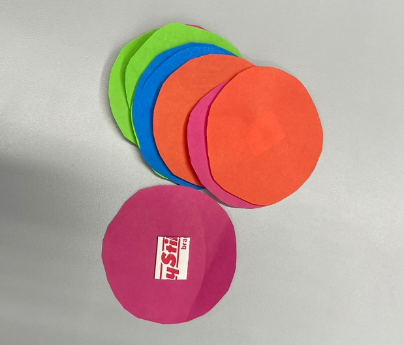
\includegraphics[width=6cm]{marcadores.png}
		\caption{hola}
		\label{2}
		\end{figure}
		
  \item Cinta
			 \begin{figure}[!h]
		\center
		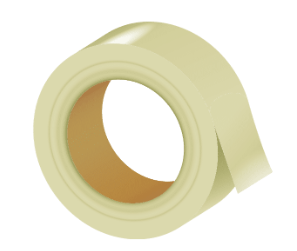
\includegraphics[width=4cm]{cinta.png}
		\caption{TEXTO AQUI}
		\label{3}
		\end{figure}
		
 \item Persona.
				 \begin{figure}[!h]
			\center
			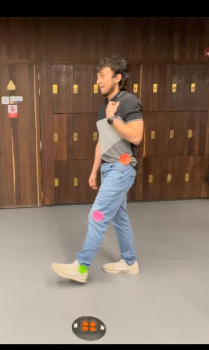
\includegraphics[width=6cm]{persona.png}
			\caption{Regla.}
			\label{4}
			\end{figure}


	\end{enumerate}


\section{Actividad Introductoria}
\begin{figure}[!h]
			\center
			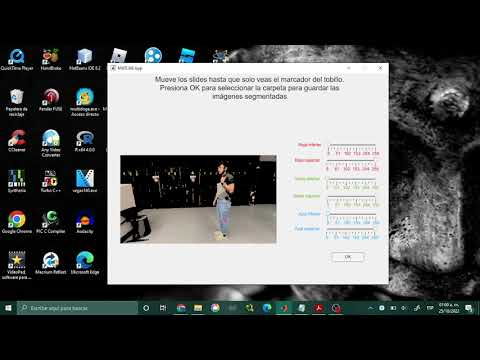
\includegraphics[width=6cm]{pantalla.jpg}
			\caption{pantalla de windows}
			\label{4}
			\end{figure}


	A los estudiantes se les solicitara hacer sus propios biomarcadores a partir de papeles de colores y se les solicitara posicionarlos en puntos clave para el análisis, en este caso: cadera, rodilla y tobillo. Posteriormente serán grabados y subidos al programa para su análisis.
	
   \section{Actividad Practica }
 
Gait Wheel:

  \begin{figure}[!h]
			\center
			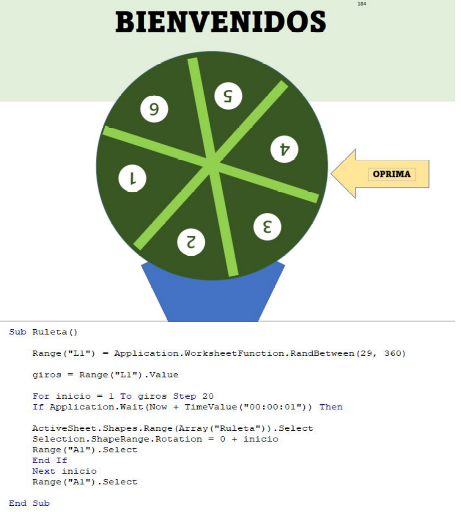
\includegraphics[width=6cm]{ruleta.png}
			\caption{ruleta + codigo}
			\label{4}
			\end{figure}
Para el desarrollo de esta actividad se optó por programar una ruleta a través de Visual Basic con sus respectivos retos cómo se muestra a continuación:
1 Salta en una pierna; 2 Baila; 3 Da largas zancadas saltando; 4 Camina lateralmente cruzando piernas; 5 Salta alternando piernas; 6 Corre abriendo y cerrando brazos.
También, como se mencionó anteriormente para la experiencia práctica, se hará uso de plask el cual es un aplicativo web desarrollado con inteligencia artificial y disponible de forma gratuita a través de internet. Nos permite extraer la posición del cuerpo humano a partir de videos y convertirlo en un formato 3D de animaciones compatible con programas como Blender. Es decir, que esta aplicación nos permite capturar la información biomecánica de la posición del cuerpo humano en un video y convertirla a un modelo computarizado en 3D que posee la animación del movimiento estudiado. Aplicaciones como estas tienen un gran impacto medico en pacientes que se benefician de los estudios biomecánicos.


PLASK: 

 \begin{enumerate}
 
 \item{Mira este video que hemos preparado para que entiendas que es Plask y cómo utilizarlo: PLASK Extracción de la posición del cuerpo humano utilizando IA}
 
   \begin{figure}[!h]
			\center
			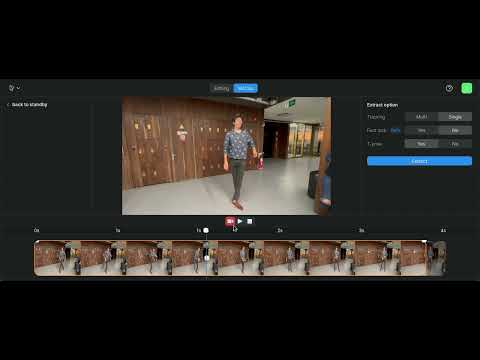
\includegraphics[width=6cm]{video.jpg}
			\caption{ruleta + codigo}
			\label{4}
			\end{figure}
			
			
 \item{ Habiendo visto el video, formen equipos de dos y elijan quien va a ser el Actor (Realiza los movimientos) y quien el productor (Graba la acción), cada uno va a tener su rol definido pero por cada turno (Giro de la ruleta) el mismo cambiara, esperen a la rotación de la ruleta y realicen la acción que les pide, ¡Cada productor será el encargado de ponerle su toque a la acción!  , recuerda el gesto debe durar entre 3 y 5 segundos y ser claro para permitir analizar el movimiento.}
 \item{Cuando el actor y productor estén de acuerdo con el gesto corporal seleccionado, graben un video que sirva para importar en el Plask, de cada uno de los integrantes del equipo}
 \item{ Realicen las animaciones y guarden un video de estas en su computador.}
 \item{Comparen las animaciones con sus compañeros de otros equipos y expliquen a que se deben las diferencias, desde un punto de vista de la mecánica del cuerpo humano.}
 
\end{enumerate}



\ifCLASSOPTIONcaptionsoff
  \newpage
\fi


\begin{thebibliography}{1}


 \bibitem{IEEEhowto:Monteria}
  Fanny Zapata. (10 de mayo de 2021). Dilatación térmica. Lifeder. Recuperado de: https://www.lifeder.com/dilatacion-termica/. 

 \bibitem{IEEEhowto:Monteria}
 La química y nosotros  (4 de Junio de 2013) Dilatación térmica en la vida cotidiana. Recuperado de: $http://katherinevaleria21.blogspot.com/2013/06/dilatacion-termica-en-la-vida-cotidiana_4.html $
\end{thebibliography}



\end{document}
